\begin{figure}[h]
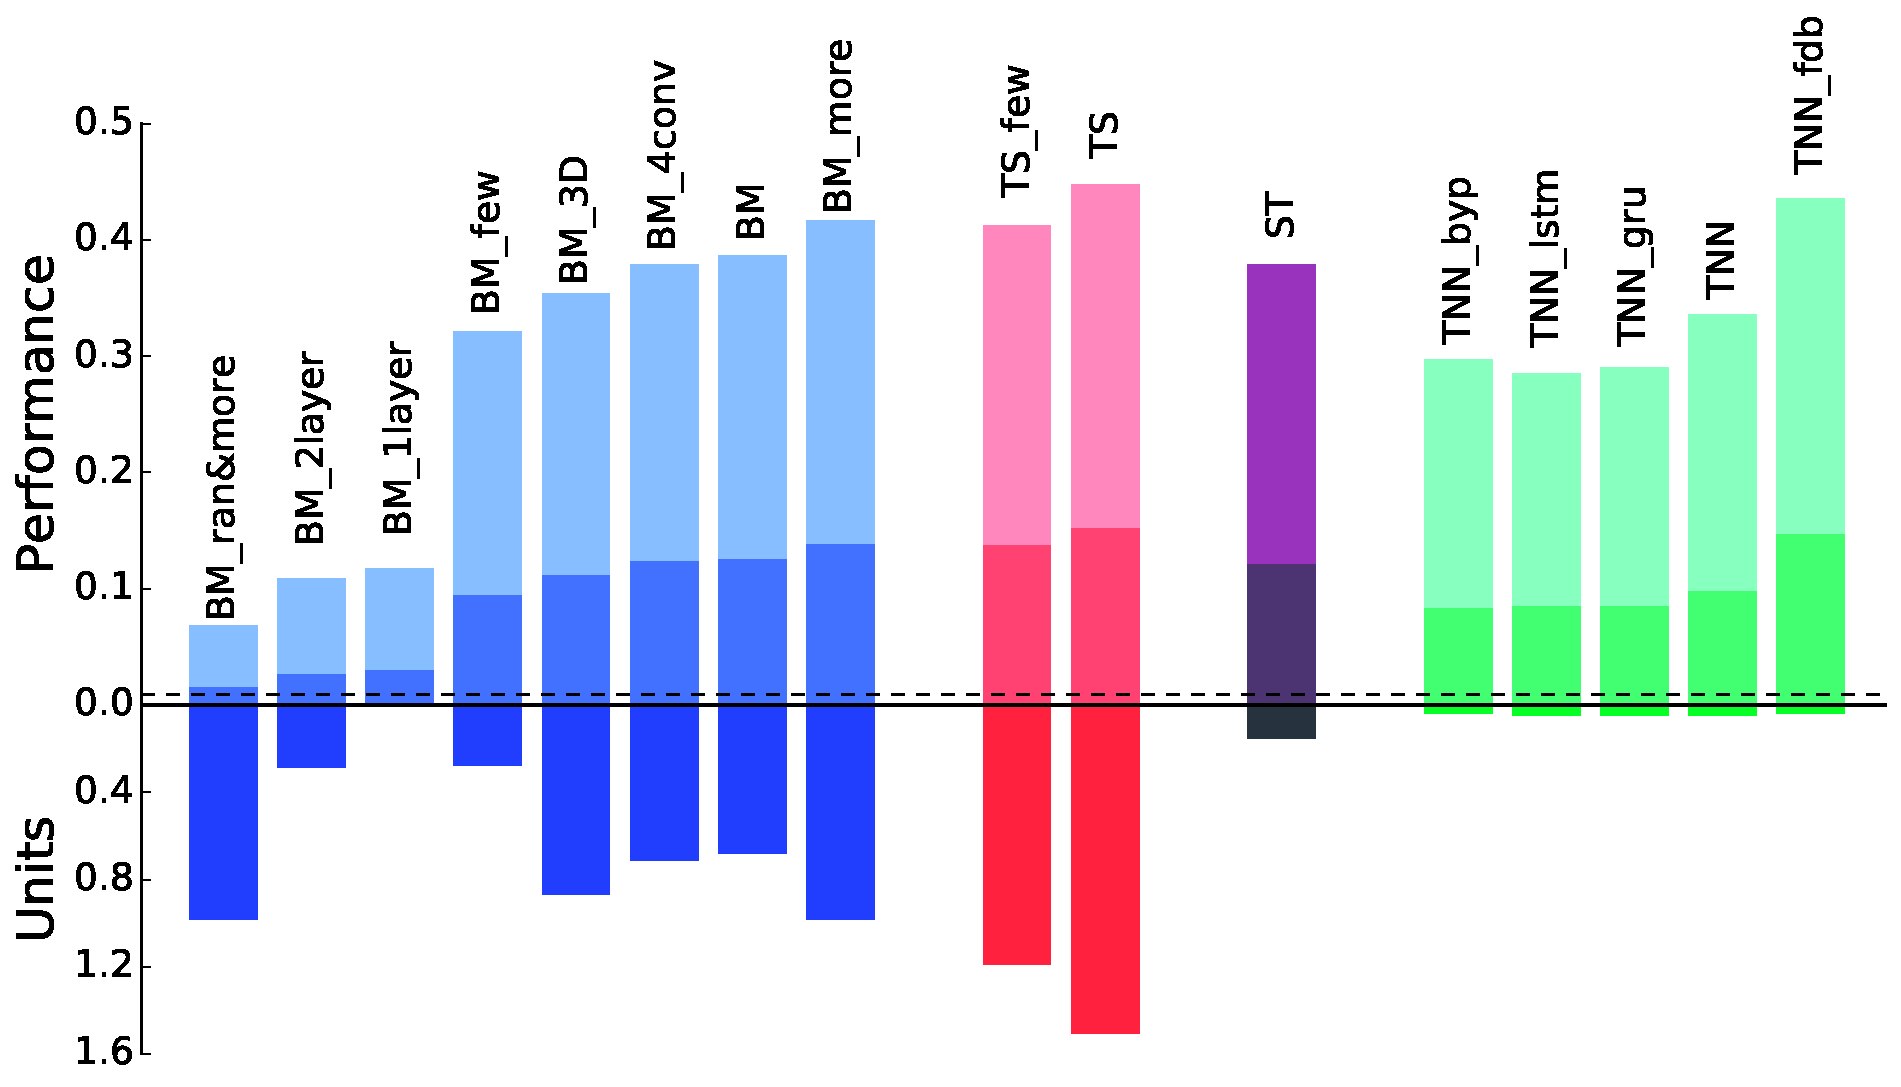
\includegraphics [width=1\linewidth]{figures/main.pdf}
\vspace{-2mm}
\caption{\textbf{Performances/number of units versus number of parameters:} Each bar in this figure represents one model. Different models in the same family have the same color and they are sorted by top1 performance in each family. The positive Y-axis is performance including top5 and top1 (in deeper color), and negative Y-axis is number of units in networks in millions. The name of each model is labeled on top of each bar. "BM", "TNN", "TS", and "ST" are the names for each family, where BM represents spatiotemporal family, TNN represents recurrent networks, TS means temporal first family, and ST means spatial first family. The meaning of these names can be found in Result section. The dash line near the bottom represents the random level of top1 performances.~\label{fig_main}}
\end{figure}

\subsection{Models in each family}

We tried many structures within each family. 
For spatiotemporal family, we tried very shallow models, having only 1 layer or 2 layers intotal in the network ("BM\_1layer" and "BM\_2layer" in Fig~\ref{fig_main}). 
We also started from the base model "BM" and varied from number of filters ("BM\_few" with fewer filters, "BM\_more" with more filters) and number of layers ("BM\_4conv" with only 4 convolution layers).
As mentioned, 3D convolution rather than 2D convolution is also tried with base model ("BM\_3D").
Besides, to show whether training is necessary, we also tried a network in the same structure of "BM\_more" with only the last output layer training while fixing the parameters of other layers as initialized ("BM\_ran\&more").
For recurrent networks, we tried models with bypass connections ("TNN\_byp"), feedback connections ("TNN\_fdb"), and LSTM or GRU recurrent cells equiped on top of it("TNN\_lstm" and "TNN\_gru").
Also, models with fewer filters are also tried for temporal first family ("TS\_few").

Realizing comparing models with different numbers of parameters trained could be unfair, we controlled that to be similar for most of the models during designing the structures. 
Specifically, the numbers of parameters trained for networks are among 22 million to 27 million, except for model "BM\_more", "BM\_few", "BM\_ran\&more" and "TS\_few", where "BM\_more" has around 83 million parameters, "BM\_few" has about 4 million paramters, "TS\_few" has 11 million parameters, and "BM\_ran\&more" only has 0.3 million parameters trained.

\subsection{Comparision between models and families}

From Fig~\ref{fig_main}, it seems that adding parameters to models can generally help the performances while number of units is not indicative of performances. 
This is much clearer when trying to compare between different families, as recurrent networks have much fewer units with similar performances as spatiotemporal family. 
More importantly, it seems that temporal first family is performing better than other families, as model "TS" has much better top1/top5 than other models with similar number of parameters.
It even performs better than "BM\_more" which has more than 3 times of parameters. 
Besides, within recurrent network family, feedback connection seems to be very important for performances, while bypass connections, LSTM or GRU cells can not help much.

In summary, it seems that performances are systematically different among families with temporal first family being the best and feedback connections is critical for recurrent networks.
